\chapter{Developmental stability of the mRNA–tRNA interface}

The results presented in this chapter are published as \citet{Schmitt:2014}.

\todo{Explain experimental design}

\todo{Remove background gradients from graphics}

In order to study how changes in \mrna gene expression relate to changes in
\trna gene expression, we collected tissue samples from six time points in mouse
development: two before birth (E15.5 and E18.5, which stands for \num{15.5} and
\num{18.5} days after gestation of the oocyte, respectively); two shortly after
birth, happening around E20 (P0.5 and P4 --- \num{0.5} and \num{4} days after
birth, respectively) and two after weaning the juvenile mice (P22 and P29). For
each of these time points, tissue was collected from whole liver and whole brain
(homogenised) and prepared for \rnaseq and \pol3 \chipseq in order to assay
\mrna and \trna gene expression. \Cref{fig:trna-project-outline} summarises the
experimental procedure.\footnote{The wet-lab work of this project was performed
by Bianca Schmitt.}

\textfig{trna-project-outline}{Sample analysis outline}{%
    Samples were collected in eight distinct time points …
}

%\section{Mouse tissue development as a model system to study mRNA and tRNA gene
%regulation}

\section{Protein-coding gene expression changes dynamically during mouse
development}

Changes in the expression of protein-coding genes, leading to changes in
abundance of proteins, are known to drive cellular behaviour\todo{ref}. Our data
confirms that tissue development in mice is accompanied by large-scale changes
to the \mrna transcriptome (\cref{fig:mrna-expression-change}).

A more systematic analysis shows that changes in gene expression happen
incrementally across the profiled stages of development: both in variance
(\cref{fig:mrna-pca}) and in the number of differentially expressed genes
between stages (\cref{fig:mrna-de-matrix}).

\spillfigure{%
    \begin{minipage}{1.2\textwidth}
        \centering
        \begingroup
            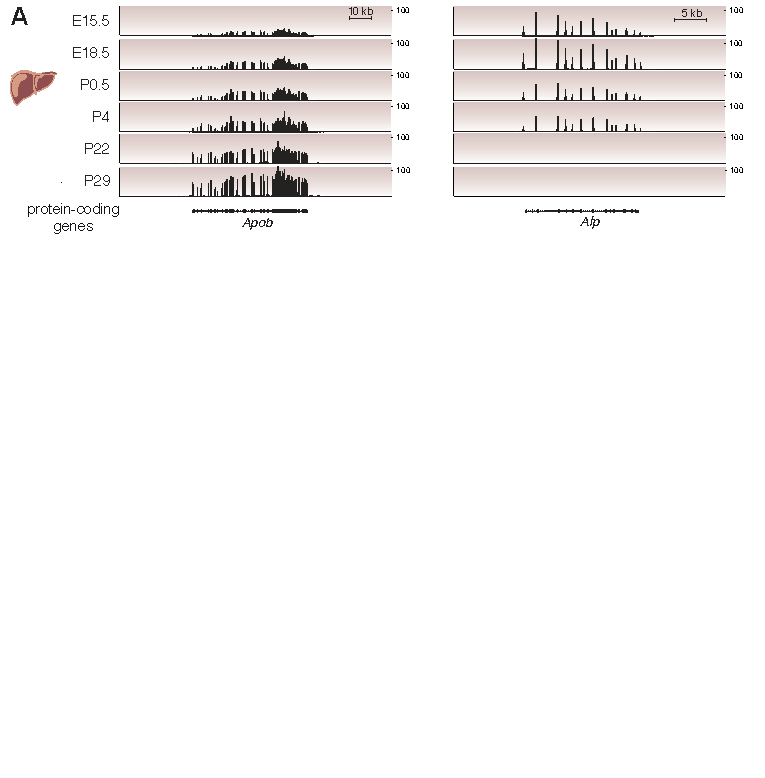
\includegraphics[width=\textwidth]{liver-mrna-expression-change}
            \subcaption{Gene expression changes of \gene{Apob} and \gene{Afp}.}
        \endgroup
        \par
        \begingroup
            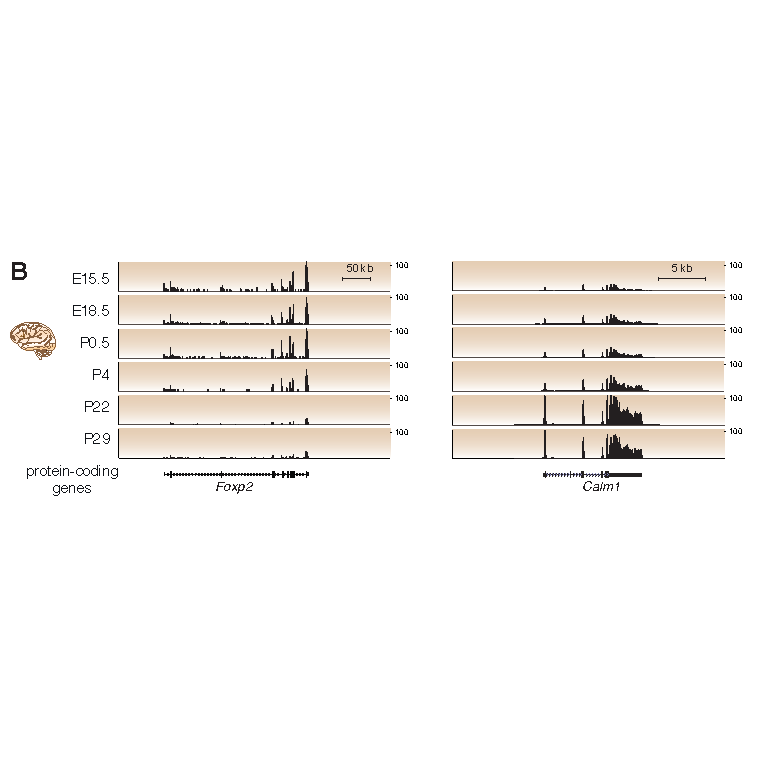
\includegraphics[width=\textwidth]{brain-mrna-expression-change}
            \subcaption{Gene expression changes of \gene{Foxp2} and \gene{Calm1}.}
        \endgroup
        \figcap{mrna-expression-change}
            {Example of gene expression changes in development.}
            {The four genes are representative for tissue- and stage-specific genes,
            whose expression changes drive cell function. These changes can go up or
            down over the course of development, correspoding to either an up- or
            downregulation.}
    \end{minipage}}

\spillfigure{%
    \begin{minipage}{0.55\textwidth}
        \centering
        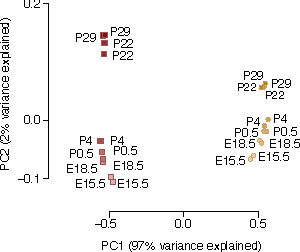
\includegraphics[width=\textwidth]{mrna-pca}
        \figcap{mrna-pca}{\pca of \mrna genes.}
            {Rotations \num{1} and \num{2} of the correlation matrix of
            protein-coding gene expressions. The percentage on the axes shows
            the amount of variance explained by each rotation.}
    \end{minipage}
    \hspace{0.1\textwidth}%
    \begin{minipage}{0.55\textwidth}
        \centering
        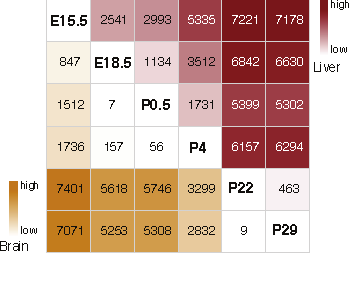
\includegraphics[width=\textwidth]{mrna-de-matrix}
        \figcap{mrna-de-matrix}
            {Number of differentially expressed \mrna genes between stages:}
            {Each off-diagonal square shows the number of differentially
            expressed genes (at a significance threshold of \(p<0.01\)) between
            the two indicated developmental stages.}
    \end{minipage}}

\section{Dynamic changes of tRNA gene expression during mouse development}

\section{Every mouse mRNA transcriptome encodes the same distribution of
triplet codons and amino acids}

\section{Stable isoacceptor anticodon abundance through development indicates
tight regulation of tRNA gene expression}

\section{mRNA triplet codon usage is highly correlated with tRNA anticodon
isoacceptor abundance during development}

\section{tRNA anticodon isoacceptor families are transcriptionally compensated
across development}
